% Options for packages loaded elsewhere
\PassOptionsToPackage{unicode}{hyperref}
\PassOptionsToPackage{hyphens}{url}
%
\documentclass[
]{article}
\author{}
\date{\vspace{-2.5em}}

\usepackage{amsmath,amssymb}
\usepackage{lmodern}
\usepackage{iftex}
\ifPDFTeX
  \usepackage[T1]{fontenc}
  \usepackage[utf8]{inputenc}
  \usepackage{textcomp} % provide euro and other symbols
\else % if luatex or xetex
  \usepackage{unicode-math}
  \defaultfontfeatures{Scale=MatchLowercase}
  \defaultfontfeatures[\rmfamily]{Ligatures=TeX,Scale=1}
\fi
% Use upquote if available, for straight quotes in verbatim environments
\IfFileExists{upquote.sty}{\usepackage{upquote}}{}
\IfFileExists{microtype.sty}{% use microtype if available
  \usepackage[]{microtype}
  \UseMicrotypeSet[protrusion]{basicmath} % disable protrusion for tt fonts
}{}
\makeatletter
\@ifundefined{KOMAClassName}{% if non-KOMA class
  \IfFileExists{parskip.sty}{%
    \usepackage{parskip}
  }{% else
    \setlength{\parindent}{0pt}
    \setlength{\parskip}{6pt plus 2pt minus 1pt}}
}{% if KOMA class
  \KOMAoptions{parskip=half}}
\makeatother
\usepackage{xcolor}
\IfFileExists{xurl.sty}{\usepackage{xurl}}{} % add URL line breaks if available
\IfFileExists{bookmark.sty}{\usepackage{bookmark}}{\usepackage{hyperref}}
\hypersetup{
  hidelinks,
  pdfcreator={LaTeX via pandoc}}
\urlstyle{same} % disable monospaced font for URLs
\usepackage[margin=1in]{geometry}
\usepackage{longtable,booktabs,array}
\usepackage{calc} % for calculating minipage widths
% Correct order of tables after \paragraph or \subparagraph
\usepackage{etoolbox}
\makeatletter
\patchcmd\longtable{\par}{\if@noskipsec\mbox{}\fi\par}{}{}
\makeatother
% Allow footnotes in longtable head/foot
\IfFileExists{footnotehyper.sty}{\usepackage{footnotehyper}}{\usepackage{footnote}}
\makesavenoteenv{longtable}
\usepackage{graphicx}
\makeatletter
\def\maxwidth{\ifdim\Gin@nat@width>\linewidth\linewidth\else\Gin@nat@width\fi}
\def\maxheight{\ifdim\Gin@nat@height>\textheight\textheight\else\Gin@nat@height\fi}
\makeatother
% Scale images if necessary, so that they will not overflow the page
% margins by default, and it is still possible to overwrite the defaults
% using explicit options in \includegraphics[width, height, ...]{}
\setkeys{Gin}{width=\maxwidth,height=\maxheight,keepaspectratio}
% Set default figure placement to htbp
\makeatletter
\def\fps@figure{htbp}
\makeatother
\setlength{\emergencystretch}{3em} % prevent overfull lines
\providecommand{\tightlist}{%
  \setlength{\itemsep}{0pt}\setlength{\parskip}{0pt}}
\setcounter{secnumdepth}{5}
\usepackage{booktabs}
\usepackage{longtable}
\usepackage{array}
\usepackage{multirow}
\usepackage{wrapfig}
\usepackage{float}
\usepackage{colortbl}
\usepackage{pdflscape}
\usepackage{tabu}
\usepackage{threeparttable}
\usepackage{threeparttablex}
\usepackage[normalem]{ulem}
\usepackage{makecell}
\usepackage{xcolor}
\ifLuaTeX
  \usepackage{selnolig}  % disable illegal ligatures
\fi

\begin{document}

\hypertarget{individual-female-aboveground-mass-and-fecundity}{%
\subsection*{Individual female aboveground mass and fecundity}\label{individual-female-aboveground-mass-and-fecundity}}
\addcontentsline{toc}{subsection}{Individual female aboveground mass and fecundity}

Individual female aboveground mass and fecundity were affected by rotation, crop species, and corn weed management (Table \ref{tab:indiv-biom-fecund-ct}). Crop identity was more influential on female aboveground mass and fecundity than corn weed management regime, but the effect of crop identity differed between corn weed management regimes (Table \ref{tab:ancova-jt}A and \ref{tab:ancova-jt}B). Differences in relative female size and fecundity across rotation by herbicide treatments were attributed to the relative size and fecundity differences when the waterhemp populations grew in different crops' presence.

Individual female aboveground mass was comparable in most pairwise comparison of the same crop species in different rotations, except S2 versus S3 (p-value = 0.0076) and S3 versus S4 (p-value = 0.0268) that followed corn under conventional weed management and C2 versus C3 (p-value = 0.0064) under low weed management. Averaged over rotations, individual female aboveground mass was 3.5- to 133.6-fold different across each pair of comparison (p-values \textless{} 0.05), except for corn under low weed management versus the succeeding oat (p-value = 0.9616).

Individual fecundity was comparable in most pairwise comparison of the same crop species in different rotations, except S2 versus S3 (p-value = 0.001) and S3 versus S4 (p-value = 0.0046) that followed corn under conventional weed management and C2 versus C3 under low weed management (p-value = 0.0032), and O3 versus O4 that followed corn under low weed management (p-value = 0.0321). Averaged over rotations, individual fecundity was comparable between corn under low herbicide and oat in the same system (p-value = 0.4904) but was 6.3- to 6857.1-fold different in other pairs of comparison (p-values \(\leq\) 0.0001).

\begin{landscape}\begin{table}

\caption{\label{tab:indiv-biom-fecund-ct}Crop and rotation system effects on individual female aboveground mass and fecundity.}
\centering
\begin{threeparttable}
\begin{tabular}[t]{lrlr>{}l|rlrl}
\toprule
\multicolumn{1}{c}{ } & \multicolumn{4}{c}{Female individual aboveground mass} & \multicolumn{4}{c}{Individual fecundity} \\
\cmidrule(l{3pt}r{3pt}){2-5} \cmidrule(l{3pt}r{3pt}){6-9}
\multicolumn{1}{c}{ } & \multicolumn{2}{c}{\makecell[c]{Conventional herbicide \\ corn weed management}} & \multicolumn{2}{c}{\makecell[c]{Low herbicide \\ corn weed management}} & \multicolumn{2}{c}{\makecell[c]{Conventional herbicide \\ corn weed management}} & \multicolumn{2}{c}{\makecell[c]{Low herbicide \\ corn weed management}} \\
\cmidrule(l{3pt}r{3pt}){2-3} \cmidrule(l{3pt}r{3pt}){4-5} \cmidrule(l{3pt}r{3pt}){6-7} \cmidrule(l{3pt}r{3pt}){8-9}
Contrast & ratio & p.value & ratio & p.value & ratio & p.value & ratio & p.value\\
\midrule
\addlinespace[0.3em]
\multicolumn{9}{l}{\textbf{(A) - Crop phase effects}}\\
\hspace{1em}C2 vs C3 & 2.62 & 0.1335 & 4.29 & 0.0064 & 3.95 & 0.0820 & 7.29 & 0.0032\\
\hspace{1em}C2 vs C4 & 2.12 & 0.3402 & 2.27 & 0.1613 & 3.00 & 0.2367 & 2.55 & 0.2288\\
\hspace{1em}C3 vs C4 & 0.81 & 0.9302 & 0.53 & 0.4070 & 0.76 & 0.9240 & 0.35 & 0.2253\\
\hspace{1em}S2 vs S3 & 0.18 & 0.0076 & 0.33 & 0.2005 & 0.07 & 0.0010 & 0.47 & 0.6323\\
\hspace{1em}S2 vs S4 & 0.70 & 0.7885 & 0.76 & 0.9068 & 0.60 & 0.7451 & 1.19 & 0.9782\\
\hspace{1em}S3 vs S4 & 3.81 & 0.0268 & 2.27 & 0.3553 & 8.45 & 0.0045 & 2.51 & 0.4525\\
\hspace{1em}O3 vs O4 & 0.93 & 0.8695 & 0.39 & 0.0457 & 0.62 & 0.4363 & 0.27 & 0.0321\\
\addlinespace[0.3em]
\multicolumn{9}{l}{\textbf{(B) - Crop species effects}}\\
\hspace{1em}soybean vs corn & 8.64 & <.0001 & 35.10 & <.0001 & 17.51 & <.0001 & 96.74 & <.0001\\
\hspace{1em}soybean vs oat & 36.55 & <.0001 & 30.29 & <.0001 & 110.44 & <.0001 & 55.97 & <.0001\\
\hspace{1em}soybean vs alfalfa & 128.16 & <.0001 & 133.62 & <.0001 & 5423.32 & <.0001 & 6857.12 & <.0001\\
\hspace{1em}corn vs oat & 4.23 & 0.0001 & 0.86 & 0.9616 & 6.31 & 0.0001 & 0.58 & 0.4904\\
\hspace{1em}corn vs alfalfa & 14.83 & <.0001 & 3.81 & 0.0099 & 309.73 & <.0001 & 70.88 & <.0001\\
\hspace{1em}oat vs alfalfa & 3.51 & 0.0324 & 4.41 & 0.0062 & 49.11 & <.0001 & 122.51 & <.0001\\
\bottomrule
\end{tabular}
\begin{tablenotes}[para]
\item \textit{Note: } 
\item C2: corn in the 2-year rotation, C3: corn in the 3-year rotation, C4: corn in the 4-year rotation, S2: soybean in the 2-year rotation, S3: soybean in the 3-year rotation; S4: soybean in the 4-year rotation, O3: oat in the 3-year rotation, O4: oat in the 4-year rotation, and A4: alfalfa in the 4-year rotation
\end{tablenotes}
\end{threeparttable}
\end{table}
\end{landscape}

\hypertarget{effects-of-weed-management-regimes-and-rotations-on-female-aboveground-mass-and-fecundity-relationship}{%
\subsection*{Effects of weed management regimes and rotations on female aboveground mass and fecundity relationship}\label{effects-of-weed-management-regimes-and-rotations-on-female-aboveground-mass-and-fecundity-relationship}}
\addcontentsline{toc}{subsection}{Effects of weed management regimes and rotations on female aboveground mass and fecundity relationship}

Since the treatment effects were statistically significant for both female aboveground mass and fecundity (Table \ref{tab:ancova-jt}), we proceeded with finding the slopes and intercepts for each linear regression of fecundity against biomass. Different slopes were specified by including interaction terms between the covariate and treatment factors. A regression slope for each treatment was necessary. That the training and testing sets' data points were well mingled indicated that the established equations were robust (Figure \ref{fig:full-p}). The equations in Table \ref{tab:ci-full} could predict waterhemp fecundity parsimoniously from dried aboveground mass using the relevant context of crop and crop management. The presented means and SEs for the estimated intercepts and slopes were established from the whole data set.

\begin{table}

\caption{\label{tab:ancova-jt}ANOVAs for effect of crop identity, corn weed management, and female aboveground mass on individual female aboveground mass (A), fecundity (B), and fecundity with aboveground mass covariate (C). Each combination of crop identity and corn weed management affected female aboveground mass and fecundity differently.}
\centering
\resizebox{\linewidth}{!}{
\begin{threeparttable}
\begin{tabular}[t]{lrrrl}
\toprule
Source of variation & df1 & df2 & F.value & p.value\\
\midrule
\addlinespace[0.3em]
\multicolumn{5}{l}{\textbf{(A) - Individual female aboveground mass. MSE = 2.02}}\\
\hspace{1em}Crop ID & 8 & 46.56 & 48.83 & <.0001\\
\hspace{1em}Corn weed management & 1 & 158.23 & 13.57 & 0.0003\\
\hspace{1em}Crop ID x Corn weed management & 8 & 73.81 & 2.36 & 0.0255\\
\addlinespace[0.3em]
\multicolumn{5}{l}{\textbf{(B) - Individual fecundity. MSE = 3.43}}\\
\hspace{1em}Crop ID & 8 & 41.61 & 72.13 & <.0001\\
\hspace{1em}Corn weed management & 1 & 146.13 & 14.64 & 0.0002\\
\hspace{1em}Crop ID x Corn weed management & 8 & 63.87 & 2.98 & 0.0067\\
\addlinespace[0.3em]
\multicolumn{5}{l}{\textbf{(C) - Individual fecundity with individual aboveground mass covariate. MSE = 1.01}}\\
\hspace{1em}Crop ID & 8 & 67.84 & 16.53 & <.0001\\
\hspace{1em}Corn weed management & 1 & 312.01 & 2.92 & 0.0886\\
\hspace{1em}Biomass & 1 & 349.08 & 483.09 & <.0001\\
\hspace{1em}Crop ID x Corn weed management & 8 & 151.00 & 1.66 & 0.1136\\
\hspace{1em}Crop ID x Biomass & 8 & 300.15 & 2.99 & 0.0031\\
\hspace{1em}Corn weed management x Biomass & 1 & 349.20 & 2.84 & 0.0931\\
\hspace{1em}Crop ID x Corn weed management x Biomass & 8 & 333.06 & 2.49 & 0.0122\\
\bottomrule
\end{tabular}
\begin{tablenotes}[para]
\item \textit{Note: } 
\item C2: corn in the 2-year rotation, C3: corn in the 3-year rotation, C4: corn in the 4-year rotation, S2: soybean in the 2-year rotation, S3: soybean in the 3-year rotation; S4: soybean in the 4-year rotation, O3: oat in the 3-year rotation, O4: oat in the 4-year rotation, and A4: alfalfa in the 4-year rotation
\end{tablenotes}
\end{threeparttable}}
\end{table}

\begin{table}

\caption{\label{tab:ci-full}Means and SEs for estimated linear regression of waterhemp fecundity (ln(seeds + 1)) versus biomass (ln(gram + 0.005)) indices intercepts and slopes, accompanied by the R$^2$ values of each equations.}
\centering
\resizebox{\linewidth}{!}{
\begin{threeparttable}
\begin{tabular}[t]{llrrrrr}
\toprule
\multicolumn{2}{c}{Effect} & \multicolumn{2}{c}{Intercept} & \multicolumn{2}{c}{Slope} & \multicolumn{1}{c}{R\$\textasciicircum{}2\$} \\
\cmidrule(l{3pt}r{3pt}){1-2} \cmidrule(l{3pt}r{3pt}){3-4} \cmidrule(l{3pt}r{3pt}){5-6} \cmidrule(l{3pt}r{3pt}){7-7}
Crop ID & Corn 
 weed management & Estimate & Std.error & Estimate & Std.error &  \\
\midrule
C2 & conv & 6.07 & 0.18 & 1.24 & 0.08 & 0.89\\
C2 & low & 5.88 & 0.22 & 1.22 & 0.11 & 0.78\\
S2 & conv & 6.30 & 0.31 & 1.14 & 0.11 & 0.89\\
S2 & low & 7.07 & 0.22 & 0.97 & 0.07 & 0.96\\
C3 & conv & 5.86 & 0.25 & 1.26 & 0.14 & 0.83\\
C3 & low & 5.11 & 0.35 & 0.66 & 0.21 & 0.33\\
S3 & conv & 7.25 & 0.44 & 0.96 & 0.09 & 0.84\\
S3 & low & 4.89 & 0.82 & 1.47 & 0.20 & 0.78\\
O3 & conv & 5.73 & 0.24 & 1.29 & 0.22 & 0.60\\
O3 & low & 5.64 & 0.21 & 0.60 & 0.18 & 0.29\\
C4 & conv & 5.90 & 0.60 & 1.26 & 0.29 & 0.60\\
C4 & low & 6.04 & 0.16 & 1.41 & 0.10 & 0.90\\
S4 & conv & 7.57 & 0.41 & 0.75 & 0.12 & 0.67\\
S4 & low & 7.33 & 0.56 & 0.74 & 0.19 & 0.58\\
O4 & conv & 6.05 & 0.18 & 1.01 & 0.16 & 0.66\\
O4 & low & 6.29 & 0.14 & 0.92 & 0.13 & 0.70\\
A4 & conv & 3.06 & 0.67 & 0.80 & 0.35 & 0.21\\
A4 & low & 1.97 & 0.43 & 0.50 & 0.20 & 0.23\\
\bottomrule
\end{tabular}
\begin{tablenotes}[para]
\item \textit{Note: } 
\item C2: corn in the 2-year rotation, C3: corn in the 3-year rotation, C4: corn in the 4-year rotation, S2: soybean in the 2-year rotation, S3: soybean in the 3-year rotation; S4: soybean in the 4-year rotation, O3: oat in the 3-year rotation, O4: oat in the 4-year rotation, and A4: alfalfa in the 4-year rotation
\end{tablenotes}
\end{threeparttable}}
\end{table}

\begin{figure}
\centering
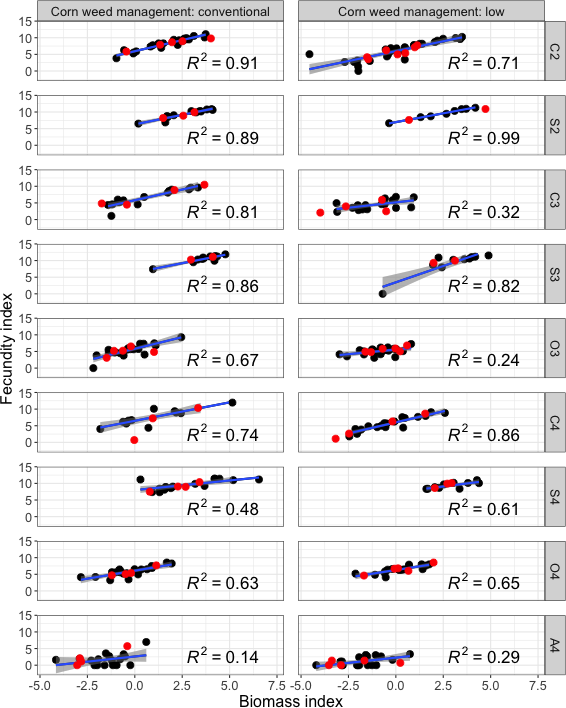
\includegraphics{Individual-fecundity-model_files/figure-latex/full-p-1.png}
\caption{\label{fig:full-p}The black and red dots are values from training and testing sets, respectively. Each regression line was plotted for one crop identity by herbicide treatment using the training set. Biomass index = ln(gram biomass + 0.005) and Fecundity index = ln(seeds + 1)}
\end{figure}

\end{document}
